\subsection{Project Finances}
\subsubsection{Bill of Materials}
Through the Senior Design class, the Calvin College Engineering department provided \$750 for prototype parts. Since the project has a large scope, the team needs to minimize the cost of any single part to stay within the given budget. As such, the team chose several parts more because of their low cost rather than for functionality. For example, the team sought donations and free samples whenever possible, including the TI MSP430 development kit from Texas Instruments and the ADE7763 power monitoring chips from Analog Devices. The Bill of Materials table shows all parts that were bought and used in final design, bought but not used in final design, and parts that were donated. 
{
\begin{longtable}[c]{|>{\centering}b{1in}|c|c|c|>{\centering}b{1in}|c|}
\caption{Materials and Cost for a Single Breaker\label{Breakers_Single.tex}}\\
\hline
\rowcolor{blue}
Item & Quantity & Unit Price & Single System & Manufacturer Part \# & Vendor \\
\hline
\endfirsthead
\caption[]{Continued from previous page}\\

\hline
\rowcolor{blue}
Item & Quantity & Unit Price & Single System & Manufacturer Part \# & Vendor \\
\hline
\endhead
\multicolumn{6}{r}{{Continued on next page}} \\
\endfoot

\endlastfoot
Solid State Relays  & 2 & 18.42 & 36.84 & STH24D25                  & Mouser \\
\hline
5pF SMD Cap         & 2 & 0.03  & 0.06  & C0603C0G1E050C            & Mouser \\
\hline
Opto Isolator       & 2 & 3.03  & 6.06  & OPI1264C                  & Mouser \\
\hline
3.579545MHz Crystal & 1 & 0.63  & 0.63  & ABLSG-3.579545MHZ-D-2-Y-T & Mouser \\
\hline
Total:              & 7 &       & 43.59 &                           &        \\
\hline
\hline
\end{longtable}
}

{
\begin{longtable}[c]{|>{\centering}b{1in}|c|c|c|>{\centering}b{1in}|c|}
\caption{Materials and Cost for 1000 Breakers\label{Breakers_Batch.tex}}\\
\hline
\rowcolor{blue}
Item & Quantity & Price per 1000 & For 1000 Systems & Manufacturer Part \# & Vendor \\
\hline
\endfirsthead
\caption[]{Continued from previous page}\\

\hline
\rowcolor{blue}
Item & Quantity & Price per 1000 & For 1000 Systems & Manufacturer Part \# & Vendor \\
\hline
\endhead
\multicolumn{6}{r}{{Continued on next page}} \\
\endfoot

\endlastfoot
Solid State Relays  & 2    & 13.00 & 26000.00 & STH24D25                  & Mouser \\
\hline
5pF SMD Cap         & 2    & 0.005 & 10.00    & C0603C0G1E050C            & Mouser \\
\hline
Opto Isolator       & 2    & 1.76  & 3520.00  & OPI1264C                  & Mouser \\
\hline
3.579545MHz Crystal & 1    & 0.35  & 350.00   & ABLSG-3.579545MHZ-D-2-Y-T & Mouser \\
\hline
Total:              & 7.00 &       & 29880.00 &                           &        \\
\hline
\hline
\end{longtable}
}

{
\begin{longtable}[c]{|>{\centering}b{1in}|c|c|c|>{\centering}b{1in}|c|}
\caption{Materials and Cost for a Single E-Meter\label{EMeter_Single.tex}}\\
\hline
\rowcolor{blue}
Item & Quantity & Part Price & Single System & Manufacturer Part \# & Vendor \\
\hline
\endfirsthead
\caption[]{Continued from previous page}\\

\hline
\rowcolor{blue}
Item & Quantity & Part Price & Single System & Manufacturer Part \# & Vendor \\
\hline
\endhead
\multicolumn{6}{r}{{Continued on next page}} \\
\endfoot

\endlastfoot
LCD Display                     & 1   & 22.75 & 22.75  & SCLBC               & SynchroSystems \\
\hline
SSOP to DIP Adapter 20-Pin      & 2   & 3.95  & 7.90   & BOB-00499           & SparkFun       \\
\hline
Break Away Headers -- Straight  & 1   & 2.5   & 2.50   & PRT-00116           & SparkFun       \\
\hline
1N4148 Diode                    & 24  & 0.09  & 2.16   & 1N4148              & Mouser         \\
\hline
2500 Series Box Header          & 2   & 1.41  & 2.82   & N2514-6002RB        & Mouser         \\
\hline
AVE Series Electrolytic Cap 1uF & 12  & 0.07  & 0.84   & AVE105M50B12T-F     & Mouser         \\
\hline
Kehmet .033uF SMD Cap           & 12  & 0.59  & 7.08   & C1206C333KARACTU    & Mouser         \\
\hline
Kehmet .015uF SMD Cap           & 6   & 0.34  & 2.04   & C1206C153KARACTU    & Mouser         \\
\hline
Kehmet 47pF SMD Cap             & 12  & 0.07  & 0.84   & C0603C470J5GACTU    & Mouser         \\
\hline
Murata Inductor EFI             & 12  & 0.11  & 1.32   & BLM21BD102SN1D      & Mouser         \\
\hline
Maxim RS233a RS232 Driver       & 1   & 8.7   & 8.70   & MAX233CPP+G36       & Mouser         \\
\hline
D-Sub 9 Connector               & 1   & 2.32  & 2.32   & 56F404-001          & Mouser         \\
\hline
Xbee Connector 2mm pitch        & 2   & 1.6   & 3.20   & M22-7131042         & Mouser         \\
\hline
16MHz Crystal                   & 1   & 0.41  & 0.41   & ABLS-16.000MHZ-B4-T & Mouser         \\
\hline
32.768kHz Crystal               & 1   & 0.99  & 0.99   & ABS10-32.768KHZ-7-T & Mouser         \\
\hline
Tyco 6P Terminal Block          & 2   & 2.33  & 4.66   & 796949-6            & Mouser         \\
\hline
Tyco 3P Terminal Block          & 2   & 0.83  & 1.66   & 796949-3            & Mouser         \\
\hline
Varistor                        & 3   & 0.26  & 0.78   & V8ZA05P             & Mouser         \\
\hline
Current Transformer             & 3   & 6.11  & 18.33  & CST-1020            & Mouser         \\
\hline
Linear Regulator                & 3   & 1.54  & 4.62   & ZSR300GTA           & Mouser         \\
\hline
100nF SMD Cap                   & 3   & 0.7   & 2.10   & CB037D0104JBA       & Mouser         \\
\hline
22uF SMD Cap                    & 4   & 0.54  & 2.16   & EEE-1CA220SR        & Mouser         \\
\hline
18pF SMD Cap                    & 2   & 0.09  & 0.18   & CGA2B2C0G1H180J     & Mouser         \\
\hline
Red SMD LED                     & 1   & 0.4   & 0.40   & HSMC-C190           & Mouser         \\
\hline
Green SMD LED                   & 1   & 0.88  & 0.88   & HSMQ-C120           & Mouser         \\
\hline
Amber SMD LED                   & 1   & 0.4   & 0.40   & HSMA-C190           & Mouser         \\
\hline
7pF SMD Cap                     & 2   & 0.03  & 0.06   & C0603C0G1E070C      & Mouser         \\
\hline
Tact Switch                     & 2   & 0.47  & 0.94   & B3W-1052            & Mouser         \\
\hline
Total:                          & 119 &       & 103.04 &                     &                \\
\hline
\hline
\end{longtable}
}

{
\begin{longtable}[c]{|>{\centering}b{1in}|c|c|c|>{\centering}b{1in}|c|}
\caption{Materials and Cost for 1000 E-Meters\label{EMeter_Batch.tex}}\\
\hline
\rowcolor{blue}
Item & Quantity & Unit Price & Single System & Manufacturer Part \# & Vendor \\
\hline
\endfirsthead
\caption[]{Continued from previous page}\\

\hline
\rowcolor{blue}
Item & Quantity & Unit Price & Single System & Manufacturer Part \# & Vendor \\
\hline
\endhead
\multicolumn{6}{r}{{Continued on next page}} \\
\endfoot

\endlastfoot
Solid State Relays  & 2 & 18.42 & 36.84 & STH24D25                  & Mouser \\
\hline
5pF SMD Cap         & 2 & 0.03  & 0.06  & C0603C0G1E050C            & Mouser \\
\hline
Opto Isolator       & 2 & 3.03  & 6.06  & OPI1264C                  & Mouser \\
\hline
3.579545MHz Crystal & 1 & 0.63  & 0.63  & ABLSG-3.579545MHZ-D-2-Y-T & Mouser \\
\hline
Total:              & 7 &       & 43.59 &                           &        \\
\hline
\hline
\end{longtable}
}

{
\begin{longtable}[c]{|>{\centering}b{1in}|c|c|c|>{\centering}b{1in}|c|}
\caption{Materials and Cost for a Single Power Supply\label{Power_Supply_Single.tex}}\\
\hline
\rowcolor{blue}
Item & Quantity & Part Price & Single System & Manufacturer Part \# & Vendor \\
\hline
\endfirsthead
\caption[]{Continued from previous page}\\

\hline
\rowcolor{blue}
Item & Quantity & Part Price & Single System & Manufacturer Part \# & Vendor \\
\hline
\endhead
\multicolumn{6}{r}{{Continued on next page}} \\
\endfoot

\endlastfoot
1000uF Cap            & 1  & 3.18  & 3.18  & TVX1J102MCD        & Mouser  \\
\hline
10u Cap               & 3  & 0.3   & 0.90  & C1206C106K9PACTU   & Mouser  \\
\hline
100n Cap              & 2  & 0.03  & 0.06  & C1608Y5V1H104Z     & Mouser  \\
\hline
47n Cap               & 1  & 0.2   & 0.20  & C1608X7S2A473K     & Mouser  \\
\hline
2.2n Cap              & 1  & 0.16  & 0.16  & 06035C222K4Z2A     & Mouser  \\
\hline
1n Cap                & 1  & 0.03  & 0.03  & C1608X7R1H102M     & Mouser  \\
\hline
2A 30V Schottky Diode & 1  & 0.55  & 0.55  & RB060M-30TR        & Mouser  \\
\hline
4.7u Inductor         & 1  & 0.72  & 0.72  & SRR0604-4R7ML      & Mouser  \\
\hline
56K Resistor          & 1  & 1.6   & 1.60  & RG1608N-563-B-T1   & Mouser  \\
\hline
15K Resistor          & 1  & 0.1   & 0.10  & TNPW060315K0DEEA   & Mouser  \\
\hline
10K Resistor          & 1  & 1.1   & 1.10  & PAT0603E1002BST1   & Mouser  \\
\hline
1.5K Resistor         & 2  & 0.79  & 1.58  & TNPW06031K50BEEN   & Mouser  \\
\hline
10 Resistor           & 2  & 0.62  & 1.24  & TNPW060310R0BEEA   & Mouser  \\
\hline
0.1 Resistor          & 1  & 0.3   & 0.30  & CRL1206-FW-R100ELF & Mouser  \\
\hline
LM25011               & 1  & 4.86  & 4.86  & LM25011MY/NOPB     & Digikey \\
\hline
Transformer           & 1  & 23.56 & 23.56 & 166M18             & Mouser  \\
\hline
Diode                 & 4  & 0.23  & 0.92  & 1N4004G            & Mouser  \\
\hline
Total:                & 25 &       & 41.06 &                    &         \\
\hline
\hline
\end{longtable}
}

{
\begin{longtable}[c]{|>{\centering}b{1in}|c|c|c|>{\centering}b{1in}|c|}
\caption{Materials and Cost for 1000 Power Supplies\label{Power_Supply_Batch.tex}}\\
\hline
\rowcolor{blue}
Part & Quantity & Price per 1000 & For 1000 Systems & Manufacturer Part \# & Vendor \\
\hline
\endfirsthead
\caption[]{Continued from previous page}\\

\hline
\rowcolor{blue}
Part & Quantity & Price per 1000 & For 1000 Systems & Manufacturer Part \# & Vendor \\
\hline
\endhead
\multicolumn{6}{r}{{Continued on next page}} \\
\endfoot

\endlastfoot
1000uF Cap            & 1  & 2.02  & 2020     & TVX1J102MCD        & Mouser  \\
\hline
10u Cap               & 3  & 0.055 & 165      & C1206C106K9PACTU   & Mouser  \\
\hline
100n Cap              & 2  & 0.007 & 14       & C1608Y5V1H104Z     & Mouser  \\
\hline
47n Cap               & 1  & 0.036 & 36       & C1608X7S2A473K     & Mouser  \\
\hline
2.2n Cap              & 1  & 0.08  & 80       & 06035C222K4Z2A     & Mouser  \\
\hline
1n Cap                & 1  & 0.006 & 6        & C1608X7R1H102M     & Mouser  \\
\hline
2A 30V Schottky Diode & 1  & 0.169 & 169      & RB060M-30TR        & Mouser  \\
\hline
4.7u Inductor         & 1  & 0.34  & 340      & SRR0604-4R7ML      & Mouser  \\
\hline
56K Resistor          & 1  & 0.37  & 370      & RG1608N-563-B-T1   & Mouser  \\
\hline
15K Resistor          & 1  & 0.072 & 72       & TNPW060315K0DEEA   & Mouser  \\
\hline
10K Resistor          & 1  & 0.472 & 472      & PAT0603E1002BST1   & Mouser  \\
\hline
1.5K Resistor         & 2  & 0.47  & 940      & TNPW06031K50BEEN   & Mouser  \\
\hline
10 Resistor           & 2  & 0.37  & 740      & TNPW060310R0BEEA   & Mouser  \\
\hline
0.1 Resistor          & 1  & 0.121 & 121      & CRL1206-FW-R100ELF & Mouser  \\
\hline
LM25011               & 1  & 2.835 & 2835     & LM25011MY/NOPB     & Digikey \\
\hline
Transformer           & 1  & 17.28 & 17280    & 166M18             & Mouser  \\
\hline
Diode                 & 4  & 0.042 & 168      & 1N4004G            & Mouser  \\
\hline
Total:                & 25 &       & 25828.00 &                    &         \\
\hline
\hline
\end{longtable}
}


\subsubsection{Board Cost}
After all the dimensions were found on the parts, the Visio drawings were done in order to try to get a minimum board size to create a PCB. The PCB price was found using PCBExpress. The team did not need to pay for the PCBs originally because that service was donated by Johnson Controls Incorporated. However, if the team were to go into production they would not have this luxury. Therefore, in order to get an accurate Bill of Materials, this cost needed to be estimated at retail price along with all of the donated parts by various organizations. 
\begin{figure}[htbp]
  \centering
  \includegraphics[height=7in]{business/b_includes/Power_Supply_board_and_key}
  \caption{Power supply board mockup, 92.5 x 95 mm.}
  \label{fig:power_supply_board_mockup}
\end{figure}
\begin{figure}[htbp]
  \centering
  \subfloat[]{\label{fig:sb_board}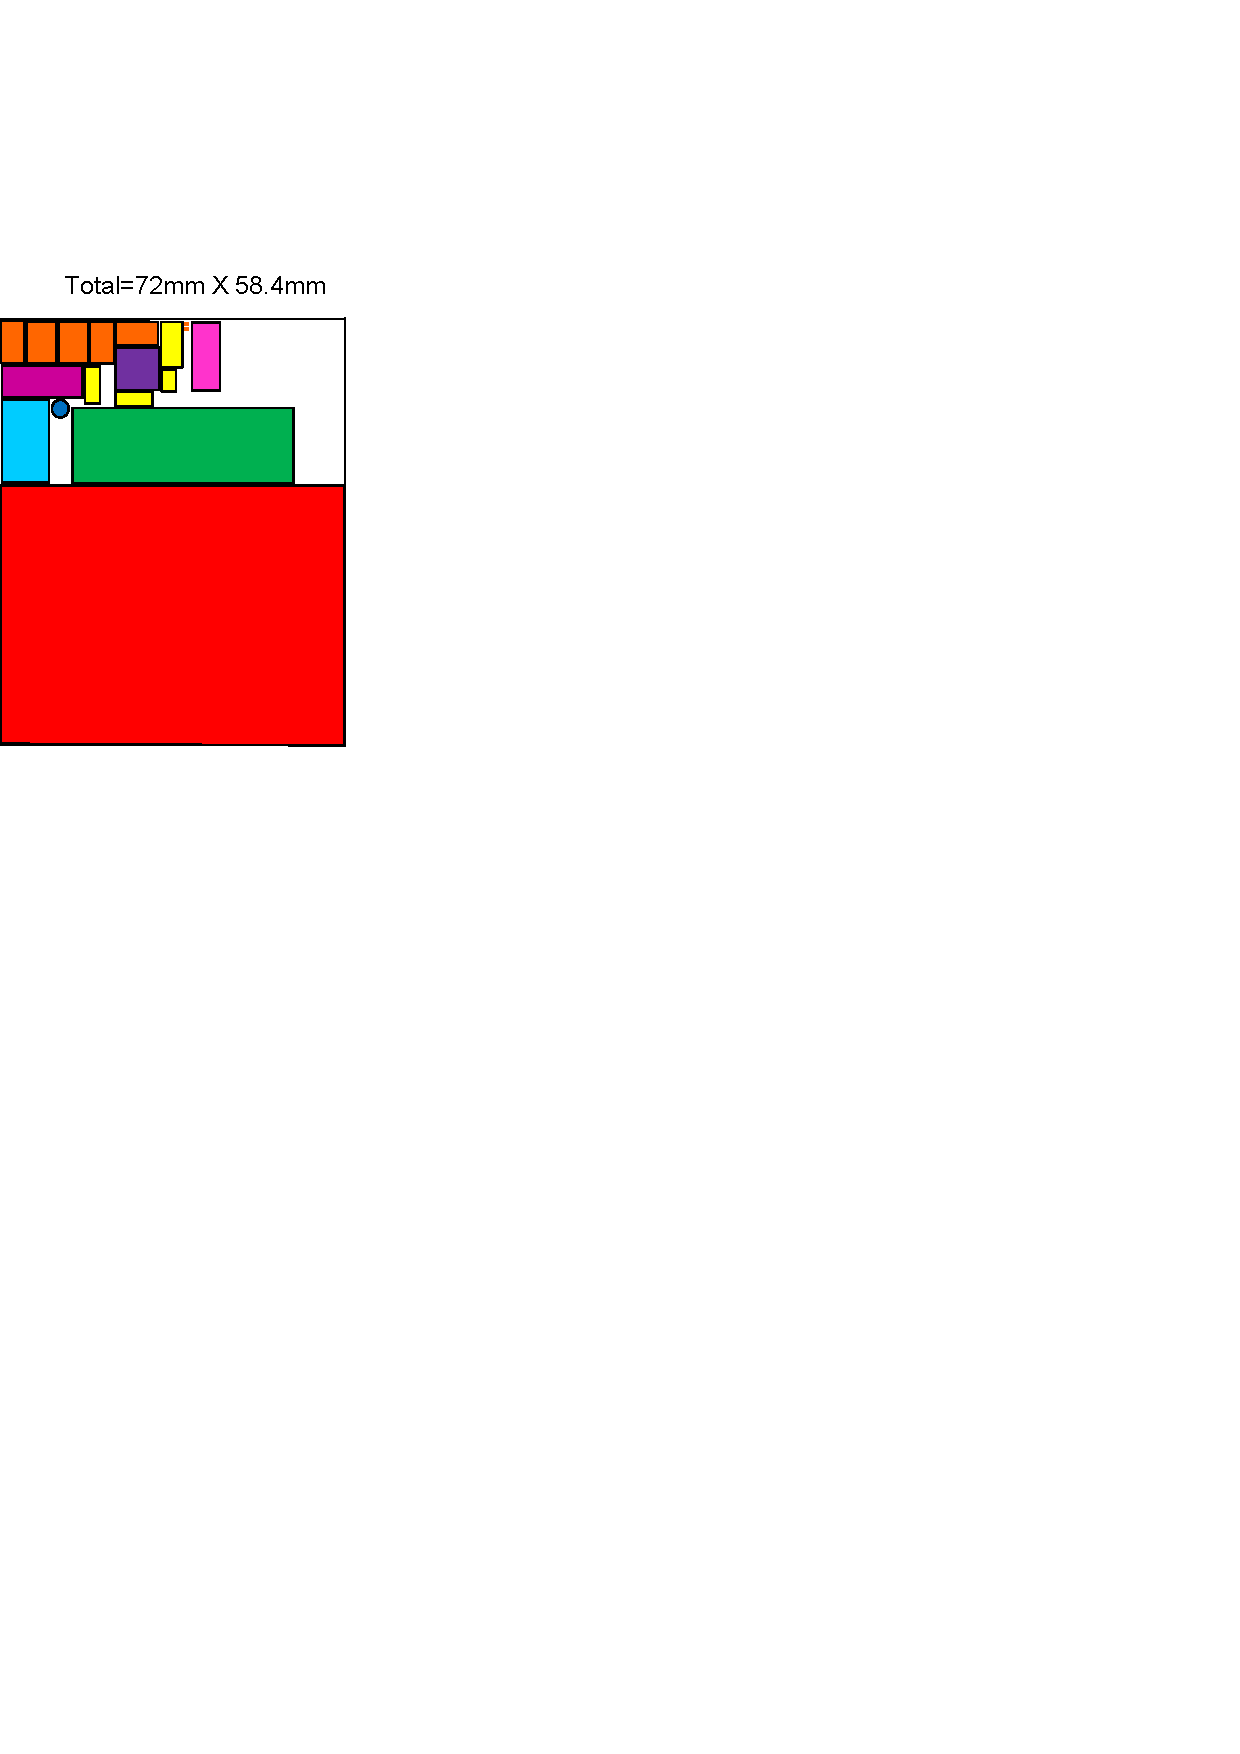
\includegraphics[width=3in]{business/b_includes/smart_breaker_board}}\\
  \subfloat[]{\label{fig:sb_key}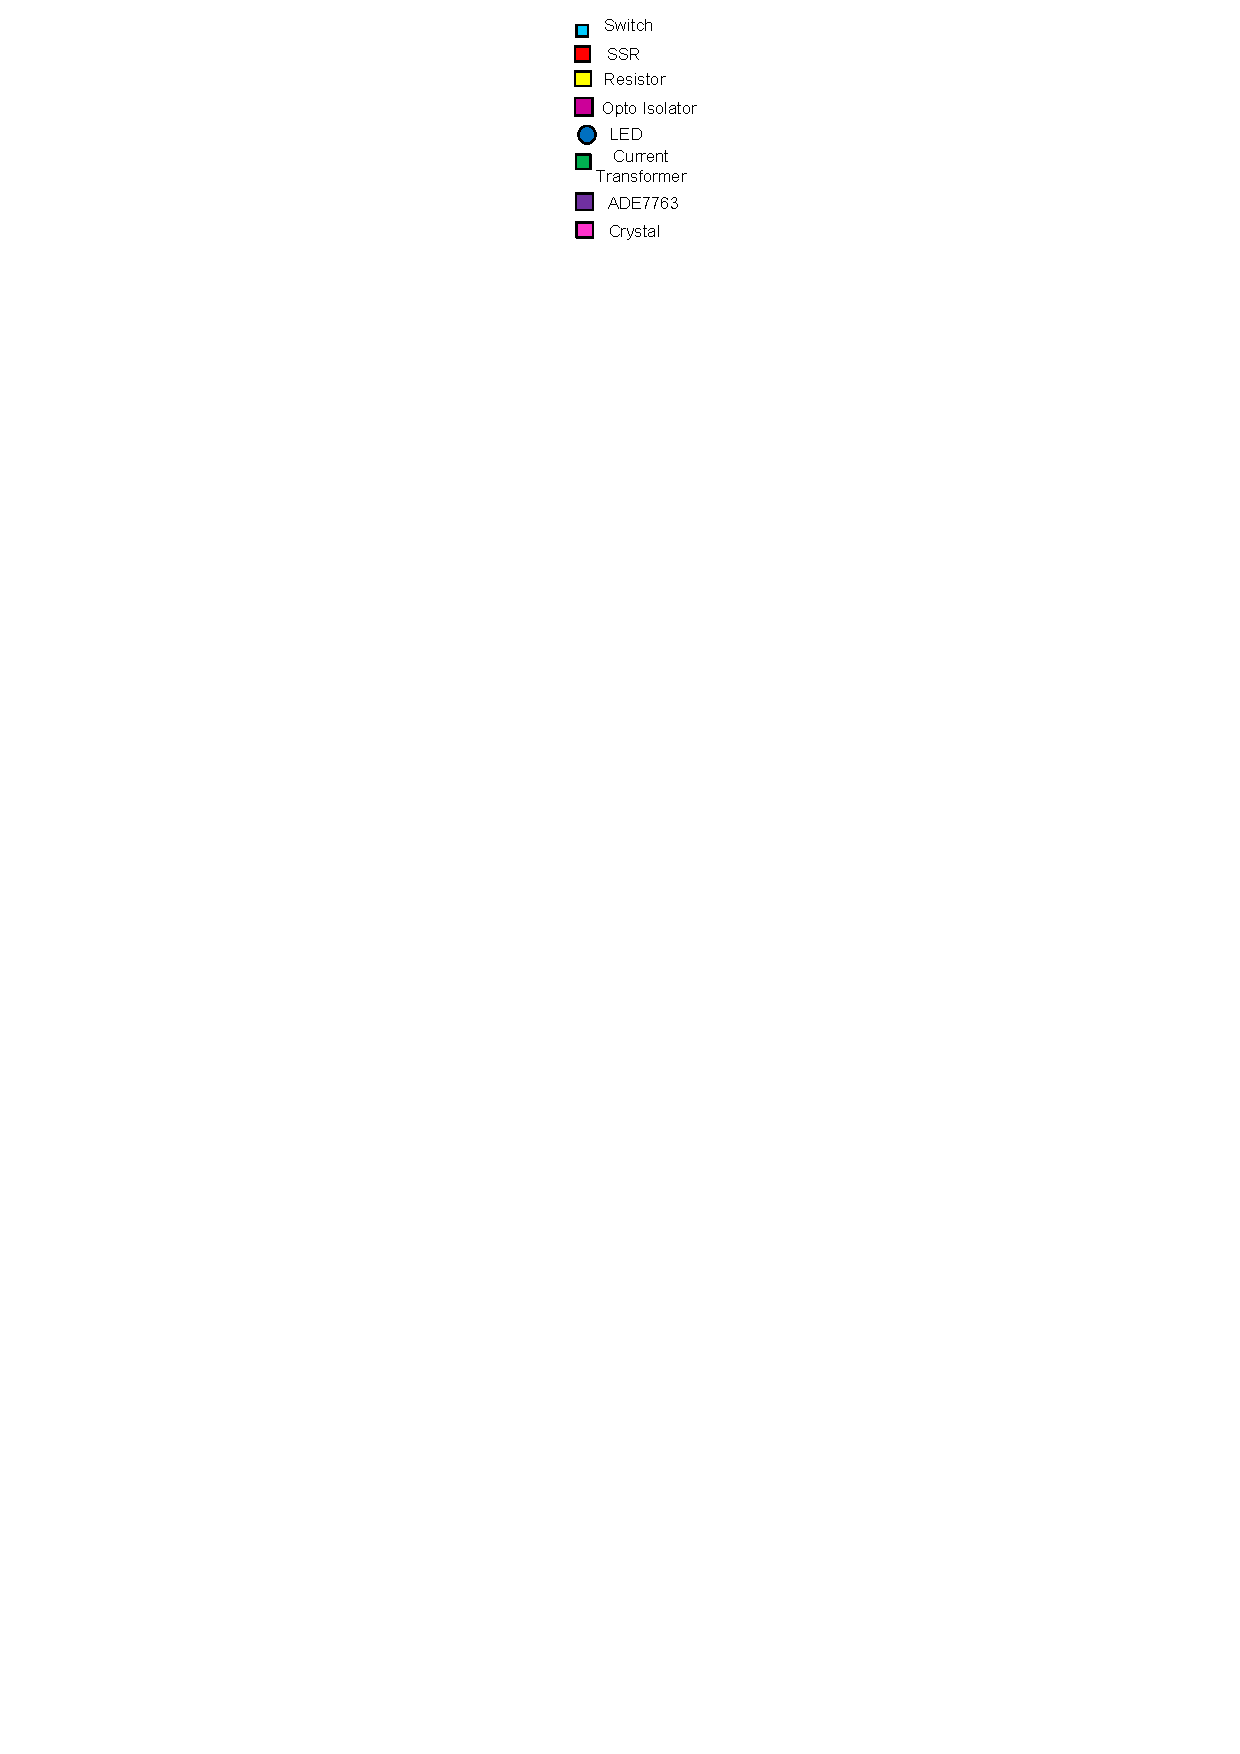
\includegraphics[width=2in]{business/b_includes/smart_breaker_key}}
  \caption{Smart breaker board mockup 72mm x 58.4mm.}
  \label{fig:smart_breaker_board_mockup}
\end{figure}
\begin{figure}[htbp]
  \centering
  \subfloat[]{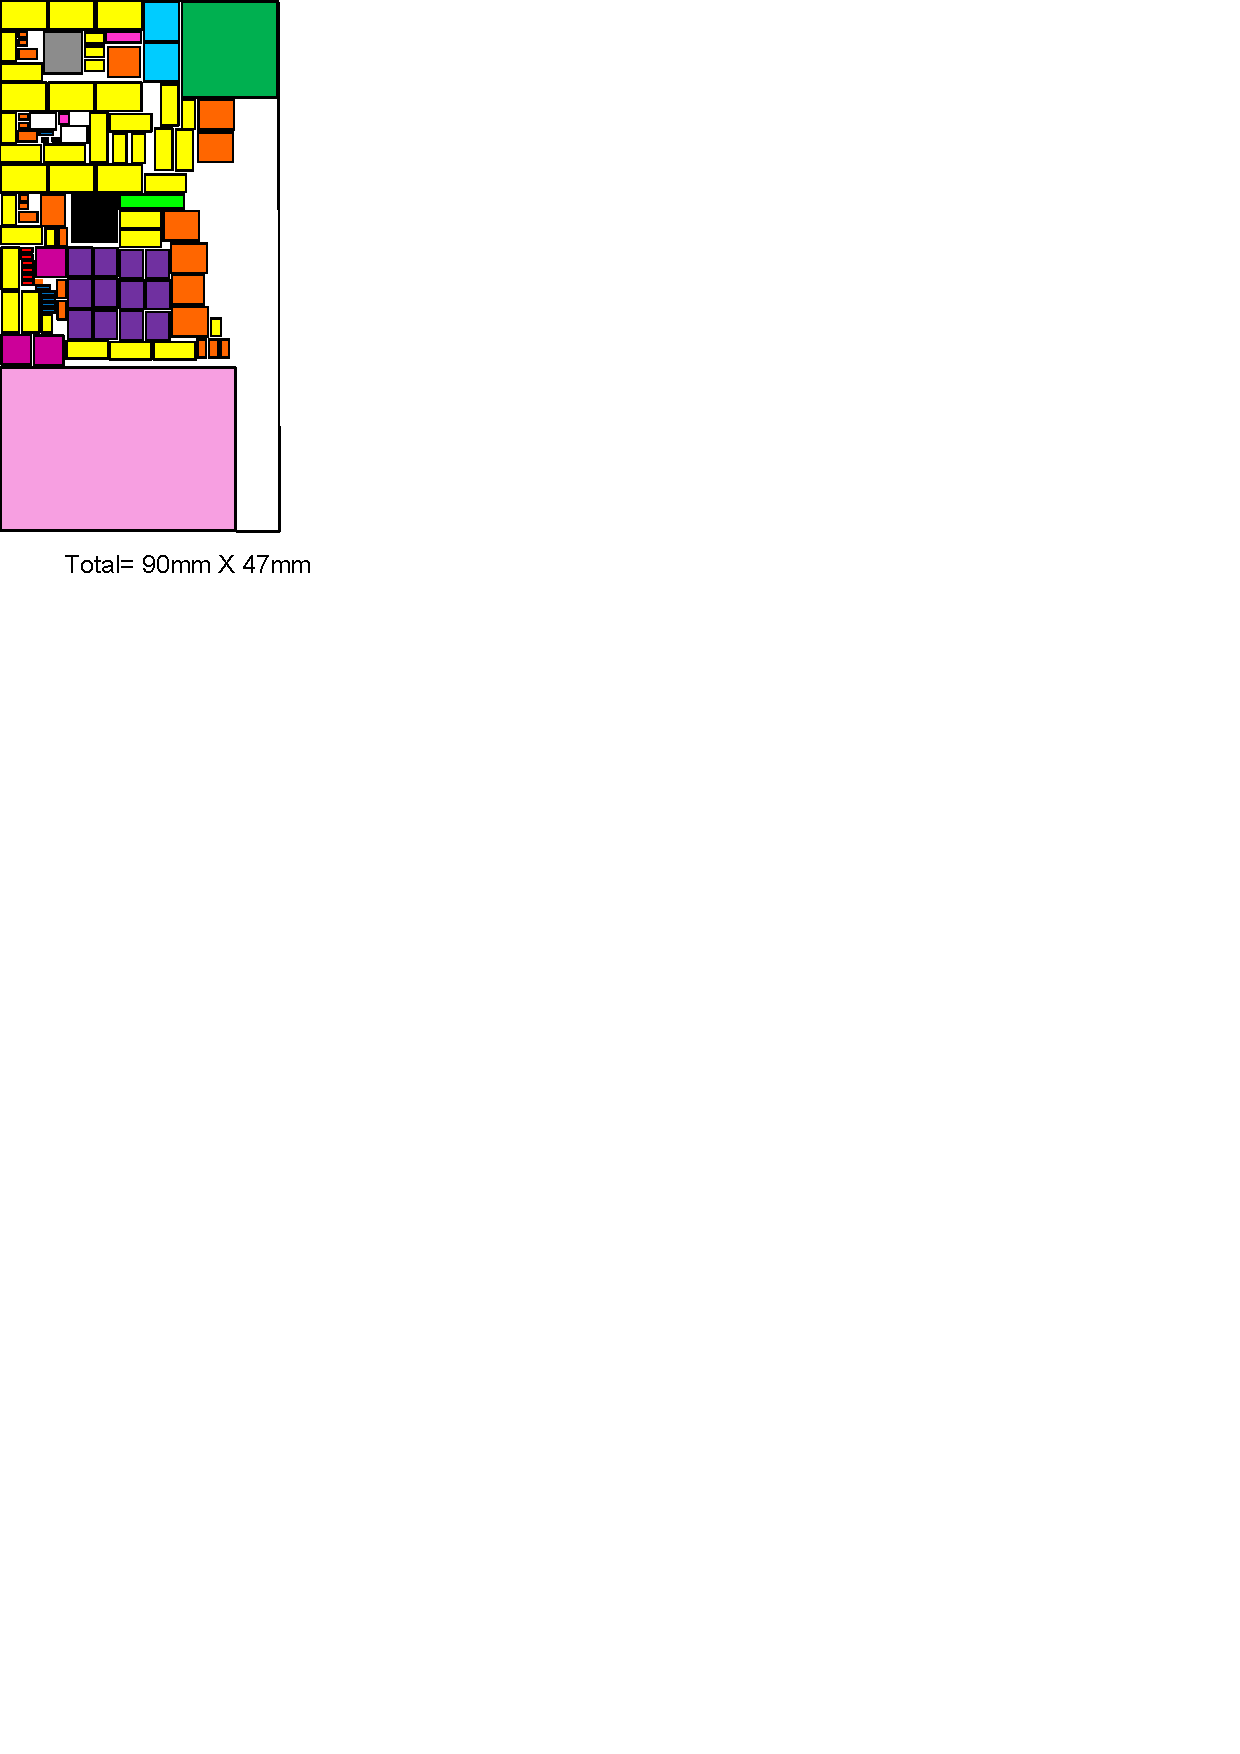
\includegraphics[height=6in]{business/b_includes/e_meter_board}}\\
  \subfloat[]{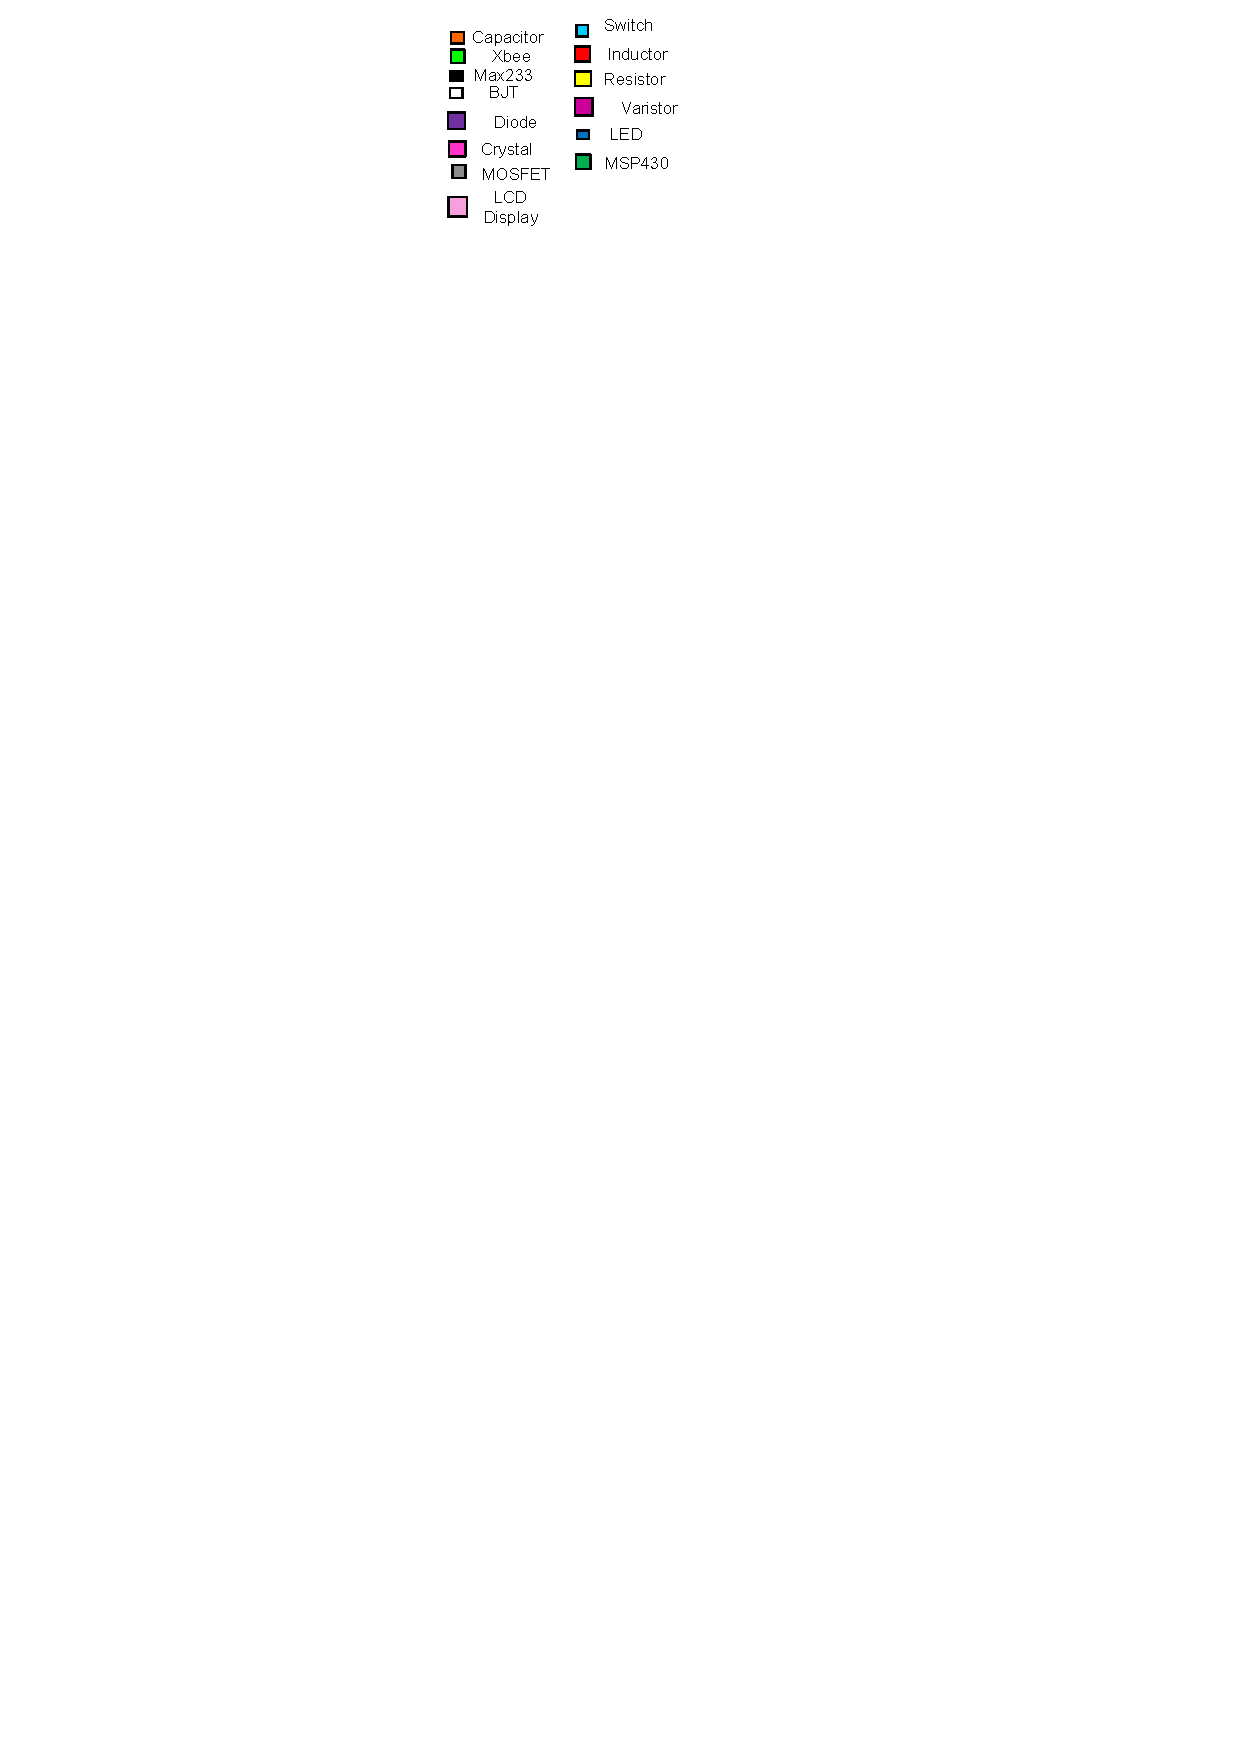
\includegraphics[width=1in]{business/b_includes/e_meter_key}}
  \caption{E-Meter board mockup 90mm x 47mm.}
  \label{fig:e_meter_board_mockup}
\end{figure}

\clearpage
\subsubsection{Labor Charges}
Throughout the first and second semester, the team has kept a log of how many hours they worked. Determining the cost of labor for both semesters can accurately be assessed based on these records. For second semester so far, the team has logged 490.75 hours, with another 127.75 estimated before the end of the semester. The team also logged 388 hours for first semester, putting the yearlong total at about 1006.5 hours. Assuming engineers are paid \$100 an hour, the first semester labor cost is \$38,800, the second semester cost is \$61,850, making the full labor costs for the project \$100,650 as calculated in table \ref{tab:projecthours}. 
\begin{table}[htbp]
  \centering
  \begin{tabular}{|c|c|c|}\hline
    \textbf{Timeframe} & \textbf{Hours Logged} & \textbf{Cost}\\\hline\hline
    First Semester     & 388                   & \$38,800\\\hline
    Second Semester    & 618.5                 & \$61,850\\\hline
    Total              & 1006.5                & \$100,650\\\hline
  \end{tabular}
  \caption{Project hours}
  \label{tab:projecthours}
\end{table}